\documentclass{cslthse-msc}
\usepackage[utf8]{inputenc}
\usepackage[english]{babel}
\usepackage{amsmath}
\usepackage{amsfonts}
\usepackage{amssymb}
\usepackage{amsthm}
%\usepackage{makeidx}
\usepackage{graphicx}
\usepackage[titletoc, header, page]{appendix}
\usepackage{hyperref}

\usepackage{float}
\usepackage{listings}

\lstset{ %
%  backgroundcolor=\color{white},   % choose the background color; you must add \usepackage{color} or \usepackage{xcolor}
  basicstyle=\footnotesize,        % the size of the fonts that are used for the code
  breakatwhitespace=false,         % sets if automatic breaks should only happen at whitespace
  breaklines=true,                 % sets automatic line breaking
  captionpos=b,                    % sets the caption-position to bottom
%  commentstyle=\color{mygreen},    % comment style
%  deletekeywords={...},            % if you want to delete keywords from the given language
  escapeinside={\%*}{*)},          % if you want to add LaTeX within your code
  extendedchars=true,              % lets you use non-ASCII characters; for 8-bits encodings only, does not work with UTF-8
  frame=single,                    % adds a frame around the code
  keepspaces=true,                 % keeps spaces in text, useful for keeping indentation of code (possibly needs columns=flexible)
%  keywordstyle=\color{blue},       % keyword style
%  language=Octave,                 % the language of the code
%  morekeywords={*,...},            % if you want to add more keywords to the set
  numbers=left,                    % where to put the line-numbers; possible values are (none, left, right)
  numbersep=10pt,                   % how far the line-numbers are from the code
  numberstyle=\tiny\color{mygray}, % the style that is used for the line-numbers
  rulecolor=\color{black},         % if not set, the frame-color may be changed on line-breaks within not-black text (e.g. comments (green here))
  showspaces=false,                % show spaces everywhere adding particular underscores; it overrides 'showstringspaces'
  showstringspaces=false,          % underline spaces within strings only
  showtabs=false,                  % show tabs within strings adding particular underscores
  stepnumber=2,                    % the step between two line-numbers. If it's 1, each line will be numbered
%  stringstyle=\color{mymauve},     % string literal style
  tabsize=2,                       % sets default tabsize to 2 spaces
  title=\lstname                   % show the filename of files included with \lstinputlisting; also try caption instead of title
}

%\geometry{showframe}

\author{
	Anton Fagerberg \\
	{\normalsize \href{mailto:ada10afa@student.lu.se}{\texttt{ada10afa@student.lu.se}}}
}

\title{Work in progress title}
\subtitle{A {\LaTeX} class}
\company{Jayway}
\supervisor{Roger Henriksson, \href{mailto:Roger.Henriksson@cs.lth.se}{\texttt{Roger.Henriksson@cs.lth.se}}}
\examiner{Görel Hedin, \href{mailto:Gorel.Hedin@cs.lth.se}{\texttt{Gorel.Hedin@cs.lth.se}}}

\date{\today}
%\date{February 18, 2014}

\acknowledgements{
If you want to thank people, do it here, on a separate right-hand page. Both the U.S. \textit{acknowledgments} and the British \textit{acknowledgements} spellings are acceptable.

We would like to thank Lennart Andersson for his feedback on this template.
}

\theabstract{
This document describes the Master's Thesis format for the theses carried out at 
the Department of Computer Science, Lund University. 

Your abstract should capture, in English, the whole thesis with focus on the problem and solution in 150 words. It should be placed on a separate right-hand page, with an additional \textit{1cm} margin on both left and right. Avoid acronyms, footnotes, and references in the abstract if possible.

Leave a \textit{2cm} vertical space after the abstract and provide a few keywords relevant for your report. Use five to six words, of which at most two should be from the title.
}

\keywords{MSc, template, report, style, structure}

%% Only used to display font sizes
\makeatletter
\newcommand\thefontsize[1]{{#1 \f@size pt\par}}
\makeatother
%%%%%%%%%%


\begin{document}
\makefrontmatter

\chapter{Performance issues with HTTP 1.1}
Hypertext Transfer Protocol (HTTP) is an application protocol for distributed, collaborative, hypermedia information systems\cite{http-info}. The first standard version of HTTP 1.1 was released in January 1997\cite{rfc2068}. The next version, HTTP/2 (originally named HTTP 2.0), is expected to be released in 2015 (ändra här om det publiceras innan ex-jobbet är klart). Although HTTP/2 addresses several of the HTTP 1.1 performance issues, it is reasonable to assume that it will take many years before HTTP/2 fully replaces HTTP 1.1 as the protocol used on all web servers and even longer for many legacy systems and clients. It is therefore relevant to  acknowledge and mitigate the performance issues related to HTTP 1.1 even many years after the HTTP/2 release.

\section{Headers}
\label{headers}

It is common in modern web applications to send a lot of HTTP requests toward a back-end API. These requests can be very small, such as an PUT request to update a single field but the actual payload can also be considered small when retrieving data from the server when it is compared to the total amount of data transmitted. Along with every HTTP request are typically plenty of headers. These headers can be a substantial part of every request and may therefore end up being the performance bottle neck if many small requests has to be transmitted.

As an example, consider the Instagram API\cite{instagram_api} which has an end-point where you can get information about a certain user account with a response serialised in JSON format. If a client was built which is supposed to show details about, for example, the 10 specific users. We can then benchmark how making 10 separate API requests would differ, in transmitted data size, from how it would behave if we could fetch all 10 users with one request.

\begin{figure}[H]
  \centering
    \begin{lstlisting}
{
    "data": {
        "id": "1574083",
        "username": "snoopdogg",
        "full_name": "Snoop Dogg",
        "profile_picture": "http://distillery...",
        "bio": "This is my bio",
        "website": "http://snoopdogg.com",
        "counts": {
            "media": 1320,
            "follows": 420,
            "followed_by": 3410
        }
    }
}
    \end{lstlisting}
  \caption{User data response from the Instagram API in JSON format.}
\end{figure}

HTTP requests can be benchmarked using cURL\cite{curl}. To make the requests authentic and look like it was made from an actual browser, we tell cURL to use the default headers provided by the browser Firefox. These headers includes among other things browsers the User-Agent, media types which are acceptable responses and so on. A local server running on port 9000 is used to simulate the the Instagram API.

\begin{figure}[H]
  \centering
\begin{lstlisting}[breaklines=true]
curl --trace-ascii - 'http://localhost:9000/user/snoopdogg' -H 'Host: localhost:9000' -H 'User-Agent: Mozilla/5.0 (Macintosh; Intel Mac OS X 10.10; rv:36.0) Gecko/20100101 Firefox/36.0' -H 'Accept: text/html,application/xhtml+xml,application/xml;q=0.9,*/*;q=0.8' -H 'Accept-Language: en-US,en;q=0.5' --compressed -H 'Connection: keep-alive' -H 'Pragma: no-cache' -H 'Cache-Control: no-cache'
\end{lstlisting}
  \caption{cURL command used in the benchmarks.}
\end{figure}

Performing this request will give us the following results:

\begin{figure}[H]
  \centering
\begin{lstlisting}[breaklines=true]
=> Send header, 355 bytes (0x163)
0000: GET /user/snoopdogg HTTP/1.1
001e: Accept-Encoding: deflate, gzip
003e: Host: localhost:9000
0054: User-Agent: Mozilla/5.0 (Macintosh; Intel Mac OS X 10.10; rv:36.
0094: 0) Gecko/20100101 Firefox/36.0
00b4: Accept: text/html,application/xhtml+xml,application/xml;q=0.9,*/
00f4: *;q=0.8
00fd: Accept-Language: en-US,en;q=0.5
011e: Connection: keep-alive
0136: Pragma: no-cache
0148: Cache-Control: no-cache
0161:
<= Recv header, 17 bytes (0x11)
0000: HTTP/1.1 200 OK
<= Recv header, 47 bytes (0x2f)
0000: Content-Type: application/json; charset=utf-8
<= Recv header, 21 bytes (0x15)
0000: Content-Length: 286
<= Recv header, 2 bytes (0x2)
0000:
<= Recv data, 286 bytes (0x11e)
\end{lstlisting}
  \caption{Results from cURL when sending an HTTP request to fetch one user. The actual response payload has been omitted.}
\end{figure}

We can from this information see that 355 bytes are sent as header data, 87 bytes are then received as header data (17 + 47 + 21 + 2) and the actual payload is 286 bytes. This means 61\% of every request to this user end-point are nothing but header data.

If we instead would expose an endpoint where all 10 users could be requested with one HTTP request which returned an array of JSON objects, we would get the following result:

\begin{figure}[H]
  \centering
\begin{lstlisting}[breaklines=true]
=> Send header, 446 bytes (0x1be)
0000: GET /users/snoopdog1,snoopdog2,snoopdog3,snoopdog4,snoopdog5,sno
0040: opdog6,snoopdog7,snoopdog8,snoopdog9,snoopdo10 HTTP/1.1
0079: Accept-Encoding: deflate, gzip
0099: Host: localhost:9000
00af: User-Agent: Mozilla/5.0 (Macintosh; Intel Mac OS X 10.10; rv:36.
00ef: 0) Gecko/20100101 Firefox/36.0
010f: Accept: text/html,application/xhtml+xml,application/xml;q=0.9,*/
014f: *;q=0.8
0158: Accept-Language: en-US,en;q=0.5
0179: Connection: keep-alive
0191: Pragma: no-cache
01a3: Cache-Control: no-cache
01bc:
<= Recv header, 17 bytes (0x11)
0000: HTTP/1.1 200 OK
<= Recv header, 47 bytes (0x2f)
0000: Content-Type: application/json; charset=utf-8
<= Recv header, 22 bytes (0x16)
0000: Content-Length: 2871
<= Recv header, 2 bytes (0x2)
0000:
<= Recv data, 2871 bytes (0xb37)
\end{lstlisting}
  \caption{Results from cURL when performing a HTTP request to fetch 10 users. The actual payload has been omitted.}
\end{figure}

From the results, we can see that the size of the sent headers has increased from 355 to 446 bytes because of the longer URL which specifies all users to fetch. The received headers are increased with just one byte from 87 to 88 because of the increased \emph{Content-Length} field. This results in a total header size of 534 bytes. The actual payload has increased from 286 bytes to 2871 bytes - about 10 fold which is expected since we request 10 users at once instead of one at a time. A very small increase in data is added because of the array-characters in the JSON format. By avoiding doing 10 separate requests and instead do one concatenated request, the overhead added because of all the headers have now been reduced from 61\% to 16\%. This number will scale with to the number of requests concatenated - the more requests concatenated, the lesser amount of overhead from HTTP headers.

\begin{figure}[H]
  \centering
    \begin{center}
      \begin{tabular}{ r | c | c }
        \textbf{\#} & \textbf{10 users, 10 request} & \textbf{10 users, 1 request} \\ \hline
        Headers & 4,420 B & 534 B \\ \hline
        Payload & 2,860 B & 2,871 B \\ \hline
        \% headers of total data & 61\% & 16\% \\ \hline
      \end{tabular}
    \end{center}
  \caption{Header and payload ratio when doing 10 separate or one concatenated request to fetch users.}
\end{figure}

The data displayed in this example should be viewed as a lower bound. In practise, HTTP cookies which are used for personalisation, analytics and session management are also sent with every HTTP request as headers and can add up to multiple kilobytes of protocol overhead for every single HTTP request\cite[page 200]{HPBN}.

This is one of the issues that may (ändra "may" om det stämmer när http2 släpps) be mitigated by using HTTP/2 which remembers which headers that has already been sent and therefore doesn't need to retransmit them on subsequent requests\cite[page 222]{HPBN}.

\section{Maximum TCP connections}
\label{max_tcp}
The HTTP 1.X protocol doesn't allow data to be multiplexed over the same connection\cite[p.194]{HPBN}. For this reason, browser vendors has introduced a connection pool of ~6 TCP connections per host (the HTTP 1.1 specification limits the pool to 2 connections\cite{rfc2616} per host, but modern browsers has refused to conform to this standard in order to decrease the load times).

A common way to deal with the connection limit is to use domain sharding. Since the limit of six TCP connections are on a host name basis, it is possible to create multiple subdomains to avoid this limit. If the subdomains \{shard1, shard2, \ldots\}.example.com where created and pointed to the same server, more than six TCP connections can be used in parallel at the same time from that machine. This approach is not without downsides as every new host requires a new DNS lookup, a TCP three-Way handshake and a slow start from TCP which can have negative impact on the load times\cite[page 199]{HPBN} - just the DNS lookup typically takes 20-120 ms\cite[page 63]{HPWS}. Another problem with domain sharding is that the browser always opens six connections per shard even if not all of them are used. In addition, domain sharding can be a complicated manual process and it is hard to calculate how many shards to use for optimal performance. When Yahoo investigated this problem they reached to conclusion that you should, as a rule of thumb, use at least two, but no more than four domain shards\cite{yahoo-performance-4}.

As an example, we can benchmark downloading thumbnails for an image gallery. Suppose we want to download 60 thumbnails, encoded in base-64 format, and the connection we are using has a lot of bandwidth but suffers from high latency.

If all images were downloaded by using a single HTTP request per thumbnail, we can see that the six TCP connection limit will become a bottleneck.

\begin{figure}[H]
  \centering
    \begin{center}
      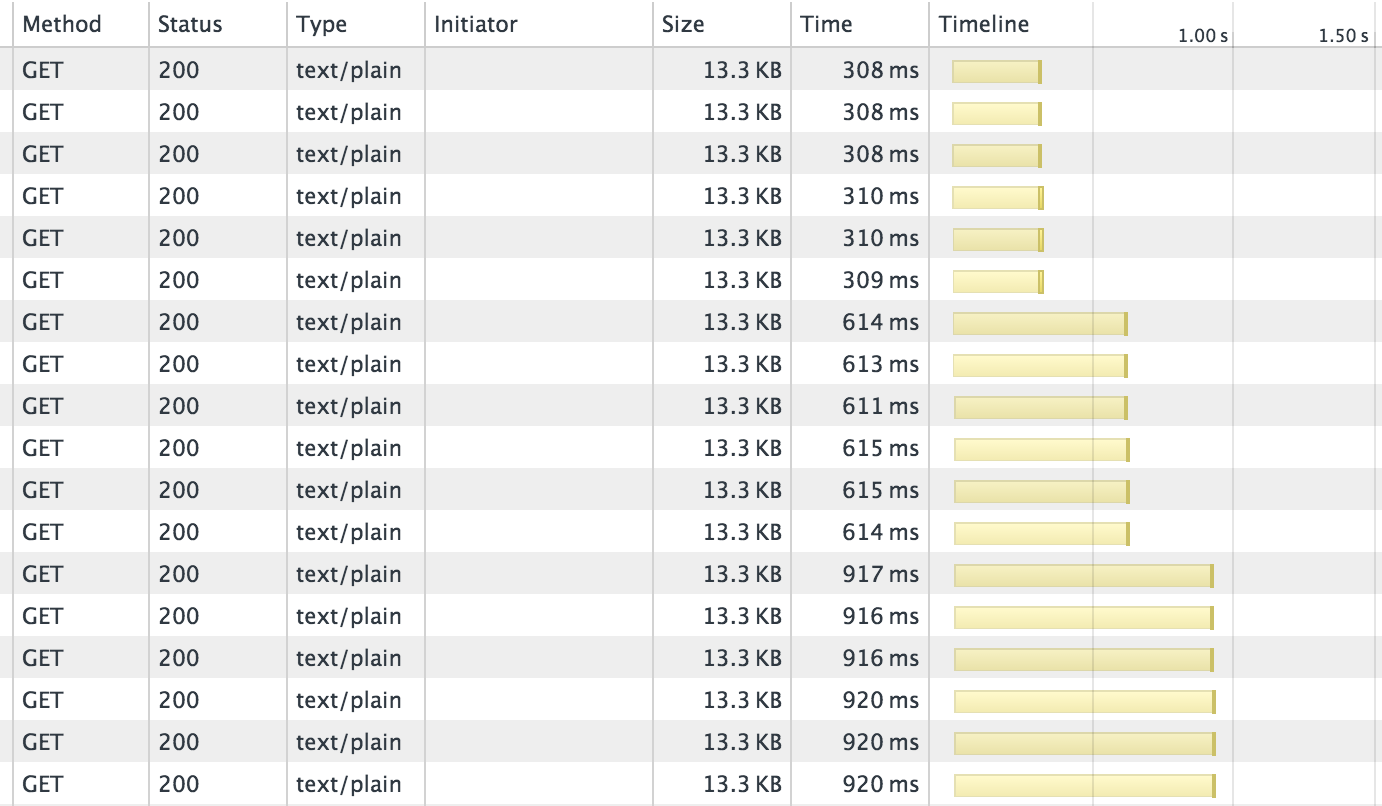
\includegraphics[width=0.9\textwidth]{images/chrome_latency_limit.png}
    \end{center}
  \caption{Chrome developer tools showing how the six TCP connection limit becomes a bottle neck on a connection with ~300 ms of latency.}
\end{figure}

We can calculate the total delay caused by latency in our example by this formula:

\begin{equation}
\mbox{total latency} = \mbox{number of thumbnails} * \frac{\mbox{latency per request}}{\mbox{number of parallel requests}}
\end{equation}

In our example, we fetch 60 thumbnails and with a latency of ~300 ms per request. Our browser can handle six parallel TCP connections which gives us the following result:

\begin{equation}
\mbox{total latency} = 60 * \frac{300}{6} = 3,000 \mbox{ ms}
\end{equation}

If we instead could concatenate these 60 thumbnail requests into one request and the response would contain all of the thumbnails - then we would only have to pay the latency cost once which would reduce the total latency by an order of magnitude from 3,000 ms to 300 ms.

It is worth pointing out that increasing the bandwidth would not resolve this problem as the latency is the only bottleneck in this scenario. It is not uncommon for browsers to wait idle for 100 - 150 ms before spending 5 ms to download an image which means that latency is accounting for 90-95\% of the total time for the HTTP requests\cite{latency}.

\subsection{Chunked responses}
When fetching thumbnails, you often want to display them as soon as each individual image has been loaded and not wait for the entire concatenated response. When using a concatenated request to fetch multiple resources at the same time, the server can use chunked transfer encoding in the HTTP response to send the thumbnail data in chunks\cite{chunked}. By doing so, images can be loaded as soon as they are available in the client, even if loaded out of order\cite{dropbox_chunked}.

\section{Compression}
\label{compression}

All requested data should be compressed before it is sent to the client. A common compression algorithm used in HTTP requests is Gzip (GNU Zip) which works best on text-based files such as HTML, CSS and JavaScript. Gzip has an expected compression rate of 60-80\% when used on text-based files\cite[page 237]{HPBN}.

It is worth mentioning that there are scenarios where Gzip compression applied to very small files can increase the total size because of the Gzip dictionary overhead. This problem can be mitigated by defining a minimum file size threshold\cite{google_gzip}.

As an example, arbitrary user data for 50 users was created and stored in JSON format. When this data was requested from the server without compression, the total content-length of the HTTP request payload amounted to 55,205 bytes. When applying Gzip compression to the same data, the content length was reduced to 16,563, which amounts to a space saving of 70\%. 

\begin{equation}
\mbox{Space Saving} = 1 - \frac{\mbox{Compressed Size}}{\mbox{Uncompressed Size}} = 1 - \frac{16,563}{55,205} = 70\%
\end{equation}

An important thing to note about Gzip compression is that only the payload is compressed in HTTP 1.1\cite{header_compression}. This means that the headers including cookies are not compressed which would've otherwise been an additional performance gain. This is one of the improvements which have been addressed in HTTP/2\cite[page 222]{HPBN}.

\chapter{API Gateways in theory}
When developing clients for a back-end API, you often find that the clients need and the APIs functionality isn't a perfect match. Different functionality is often required based on whether the client is a mobile application, a desktop application or something entirely different. The way the clients want to use the API can also radically differ. Not being able to optimise the API for each clients need can hurt the clients performance which has to do a lot of extra work but can also strain the developer whom may have to do extra work to fit the API for every client. One approach to solve this problem is by utilising an API gateway.

\section{What is an API Gateway?}
An API gateway works as an additional layer between the client and the server. For an API gateway to be efficient, it has to be able to augment the communication between the client and the server, and by doing so, improve the client performance and developer implementation of it.

\begin{figure}[H]
  \centering
    \begin{center}
      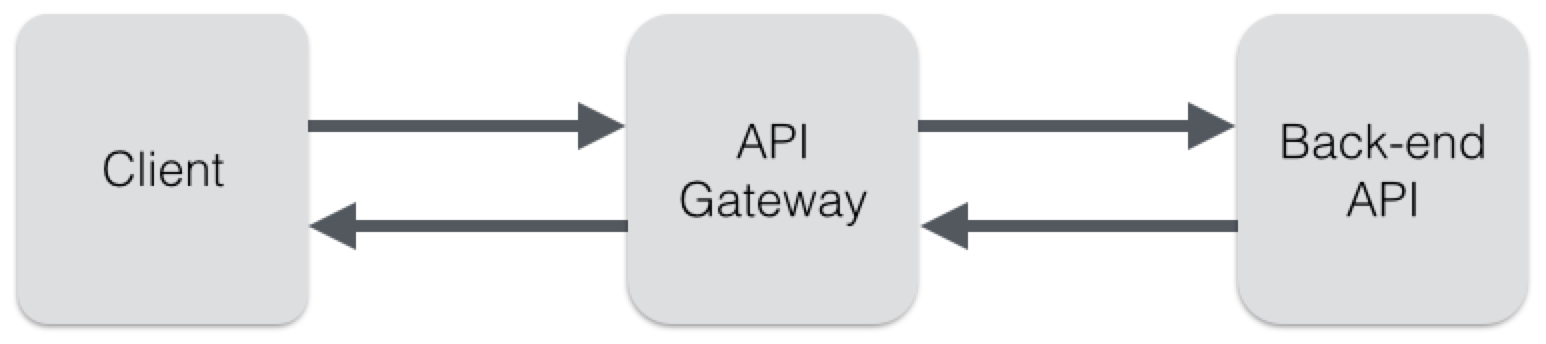
\includegraphics[width=0.9\textwidth]{images/api_gateway.png}
    \end{center}
  \caption{A simple scenario using an API gateway between a client and a back-end API.}
\end{figure}

\section{Multiple resources \& requests}
A client often has to perform many requests simultaneously, either to one or multiple back-end APIs. Typical scenarios are when a user loads a web application for the first time and the applications initial state and data has to be retrieved or when multiple connected resources has to be loaded.

\begin{figure}[H]
  \centering
    \begin{center}
      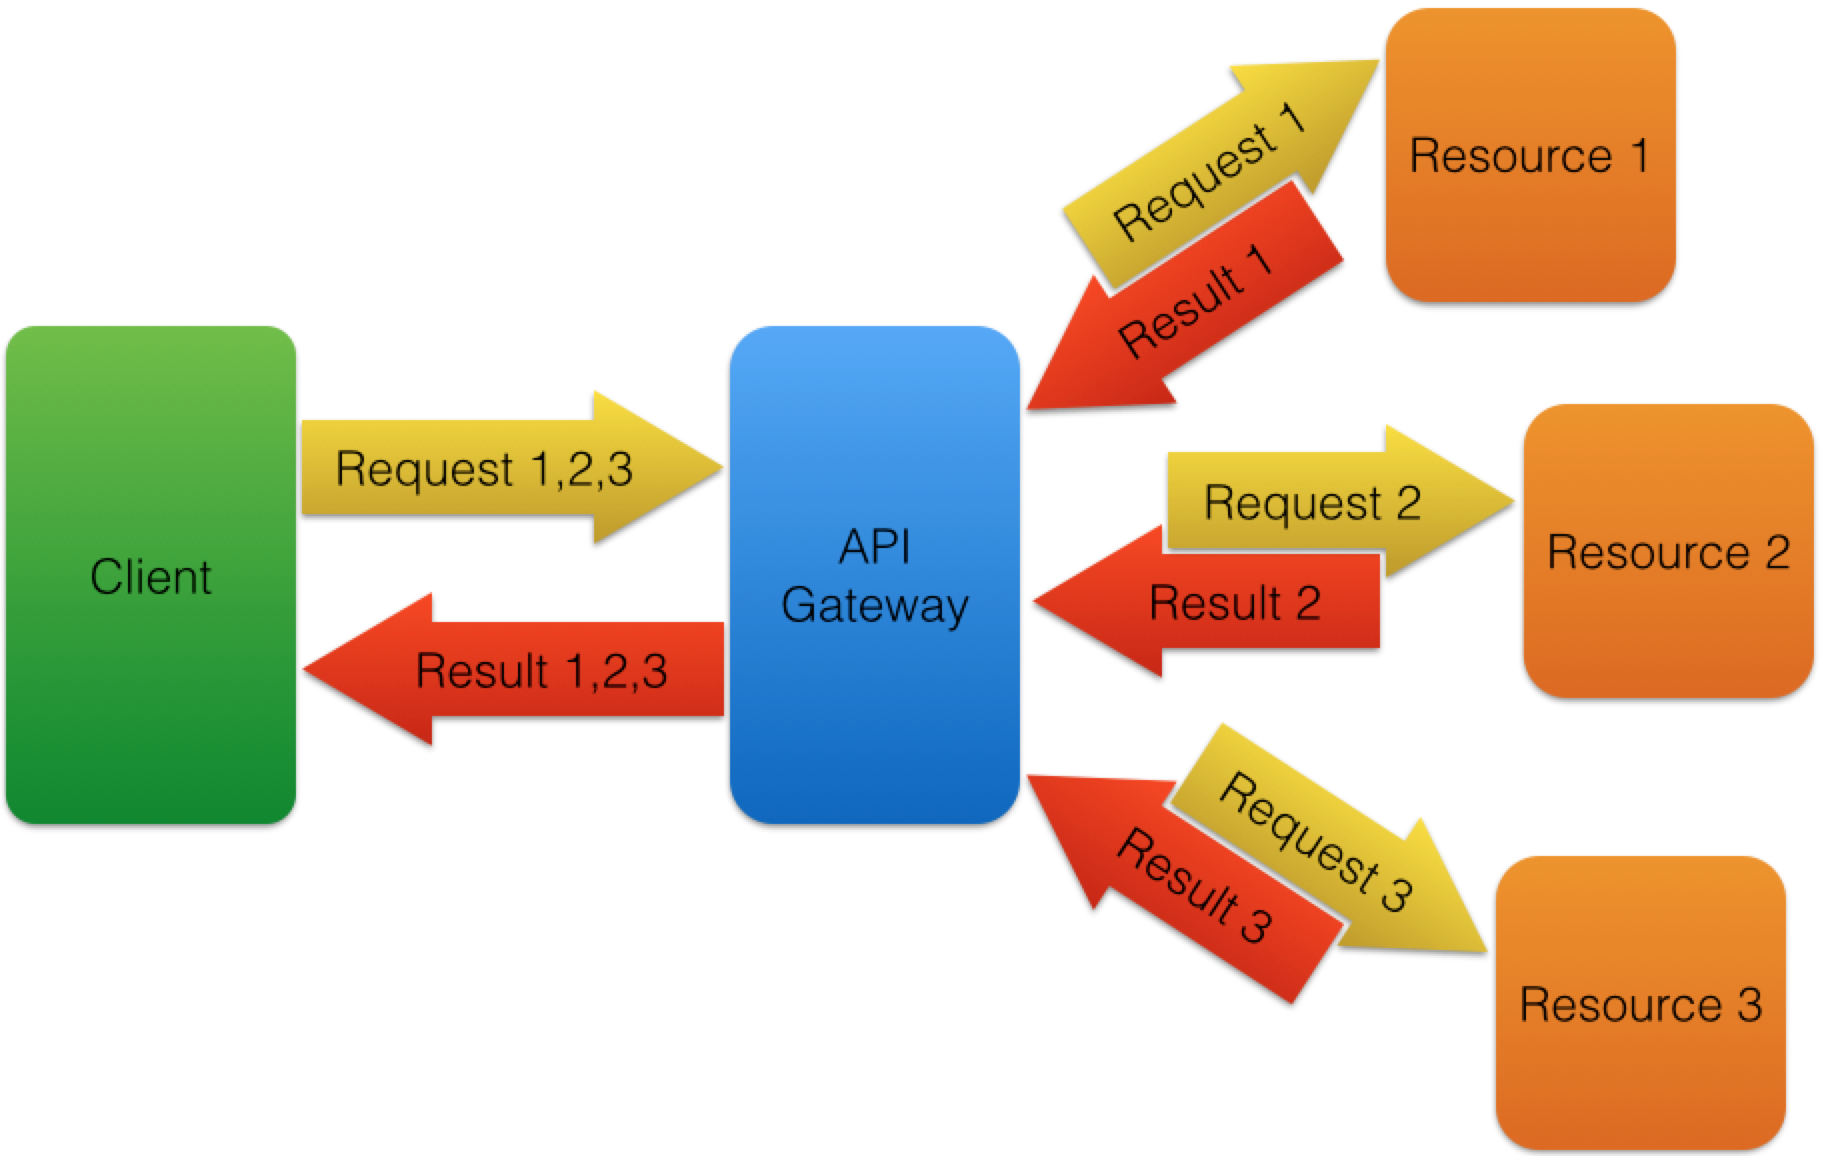
\includegraphics[width=0.9\textwidth]{images/api_gateway_concatenation.png}
    \end{center}
  \caption{An API gateway receives a concatenated request which it distributes to multiple resources, the responses are then concatenated into a single response. The resources can either be one or several back-end APIs.}
\end{figure}

When working with HTTP requests, there are multiple penalties for executing many small requests compared to one concatenated request. These penalties includes the previously mentioned limit of maximum TCP connections (page \pageref{max_tcp}) and overhead from http headers (page \pageref{headers}).

\section{Duplicate \& Unnecessary items}
When requesting data from a back-end API, the response may contain unnecessary data which the client doesn't want. In a similar fashion, if a client performs several similar requests, it is possible the all the responses contains some duplicate data. By using an API gateway, the results from the back-end API(s) can be augmented to better fit the individual clients needs.

\begin{figure}[H]
  \centering
    \begin{center}
      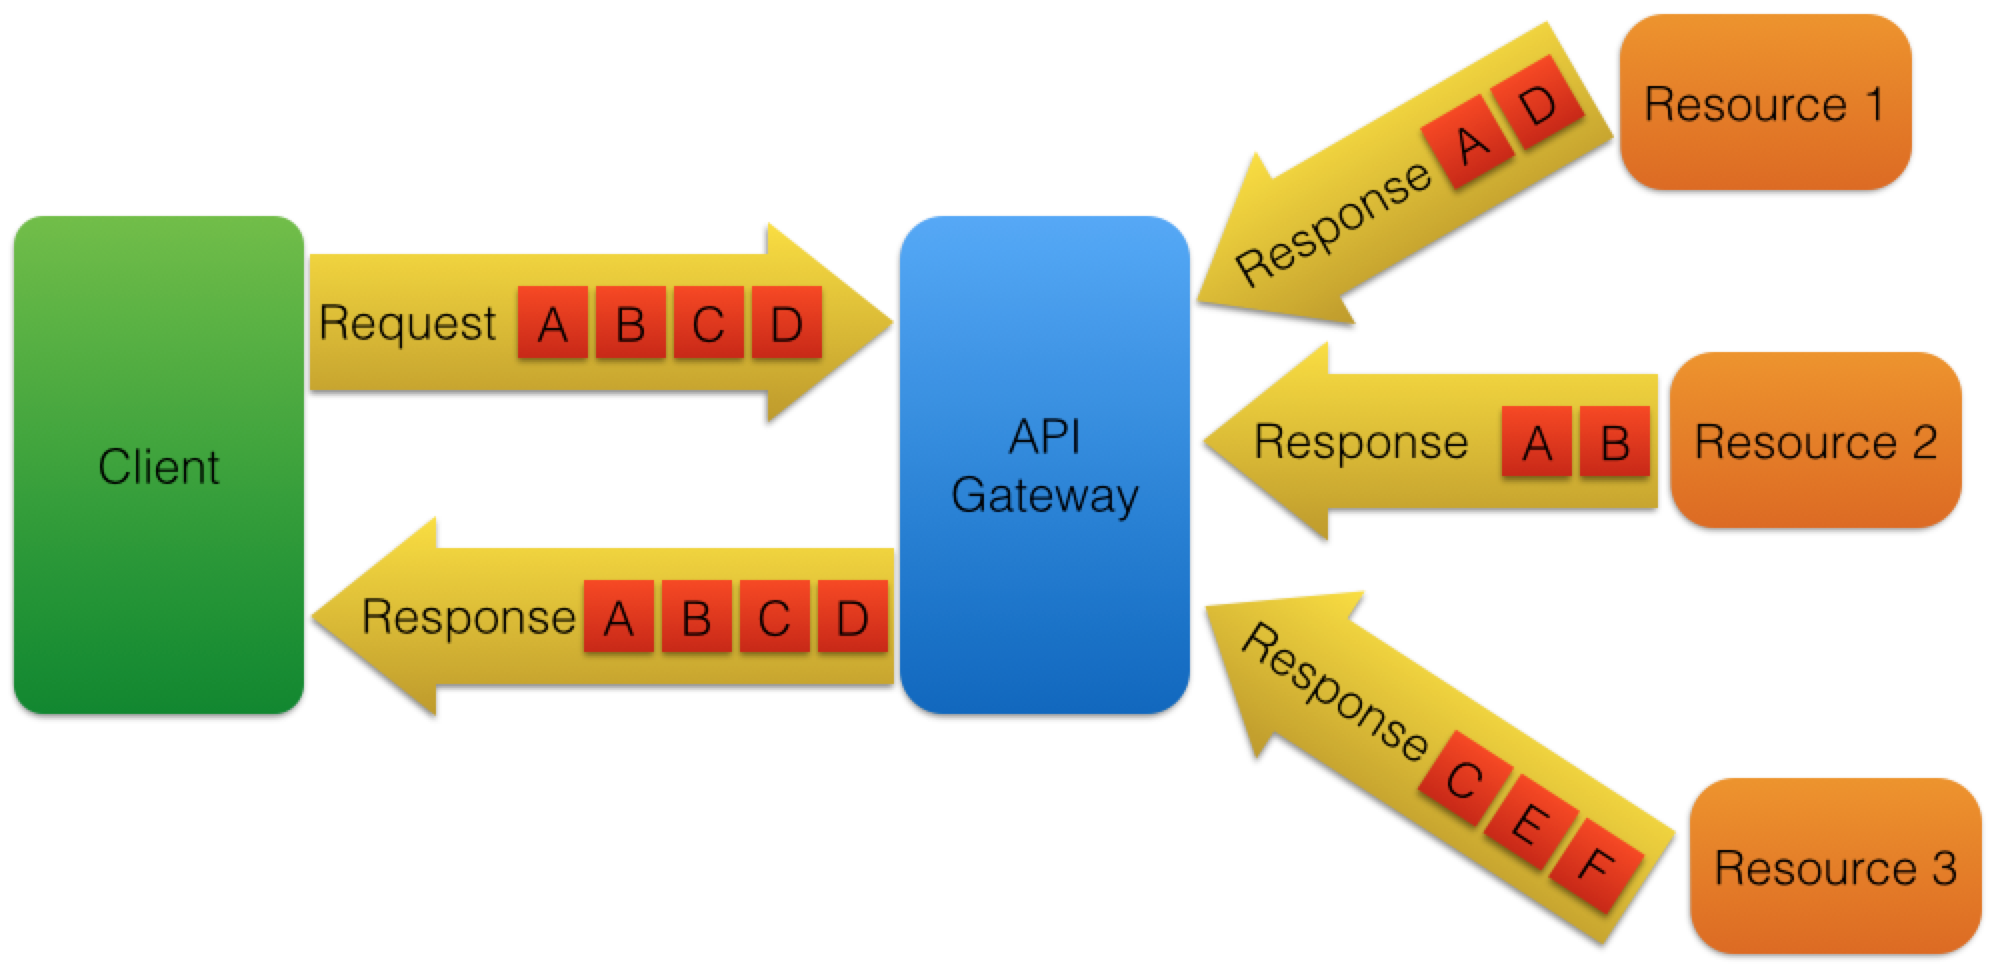
\includegraphics[width=0.9\textwidth]{images/api_gateway_duplicate.png}
    \end{center}
  \caption{Client requests item A, B, C, D. The API gateway fetches A, D from Resource 1. Item A from the Resource 2 response can be discarded since it's duplicate data. Item E, F from Resource 3 can be discarded since they are unnecessary. The API gateway can after retrieval respond with just A, B, C, D. The resources can either be one or several back-end APIs.}
\end{figure}

\section{Format transformation}
It is common when working with older legacy systems that the data is formatted in a way which is not suitable for modern clients. In the case of JavaScript, the browsers have excellent built in support for JSON but not for XML. An API gateway can on the fly convert the data from the back-end to a format more appropriate for the client and respond with it.

\begin{figure}[H]
  \centering
    \begin{center}
      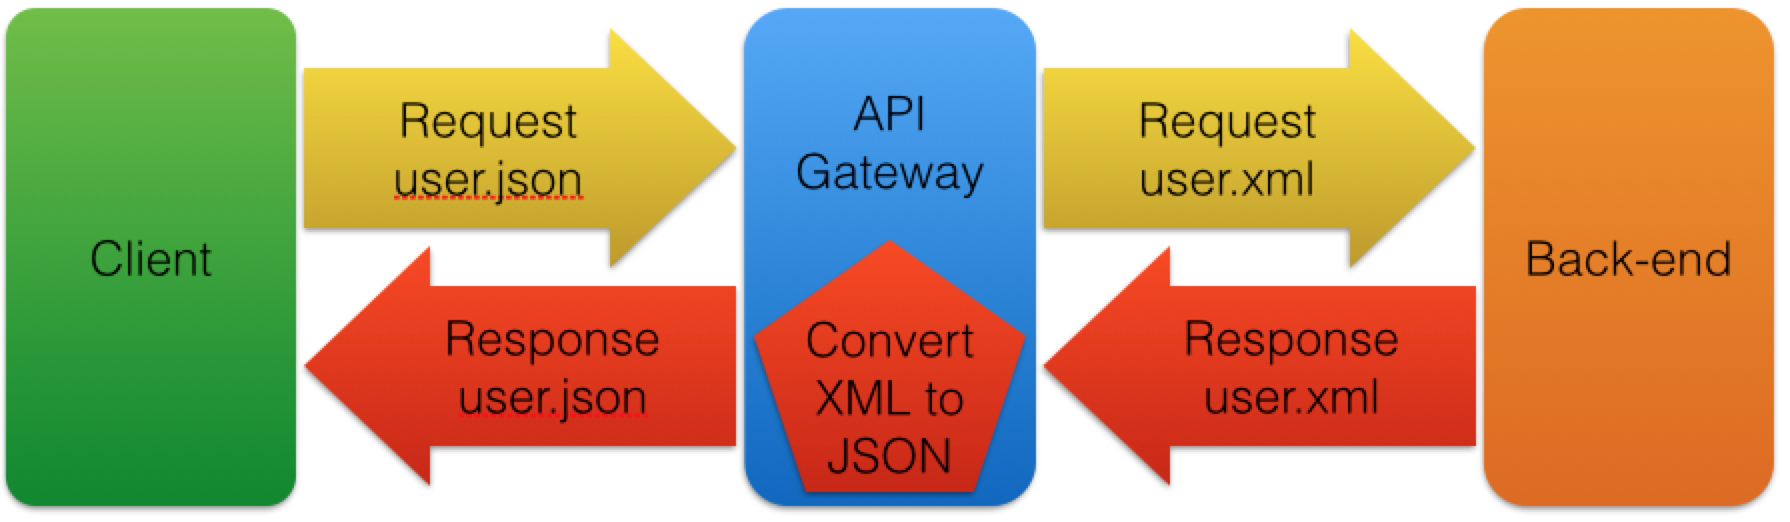
\includegraphics[width=0.9\textwidth]{images/api_gateway_transform.png}
    \end{center}
  \caption{The client requests "user" in JSON-format. The API gateway fetches "user" in XML-format from the back-end, converts it to JSON and responds to the client in the appropriate format.}
\end{figure}

This has the benefit that the conversion code doesn't has to be rewritten for different types of clients. By performing the transformation in the gateway, the processing load is moved away from the client which can improve its performance.

\section{Pure REST}
If an API follows the strict rules of REST, it uses the concept of Hypermedia as the Engine of Application State (HATEOAS). Instead of defining a bunch of end-points which the client can utilise, it requires the client to discover the resources itself by first performing a GET request to the root. To root will respond with the resources available, such as users. The client then has to query the users root to discover which requests can be made in regards to users - and so on. Working in this pure way places a very high bar for the client developer\cite[page 61]{AASG}.

API gateways can be used to transform a Pure REST API with HATEOAS to a simpler API which only follows some of the restrictions put in place by REST. This can significantly lower the amount of traffic between the client and the back-end which can be a big performance gain in cases such when the latency is high between the client and back-end (assuming that the latency between the API gateway and back-end is low such as when they are placed in the same LAN).

\begin{figure}[H]
  \centering
    \begin{center}
      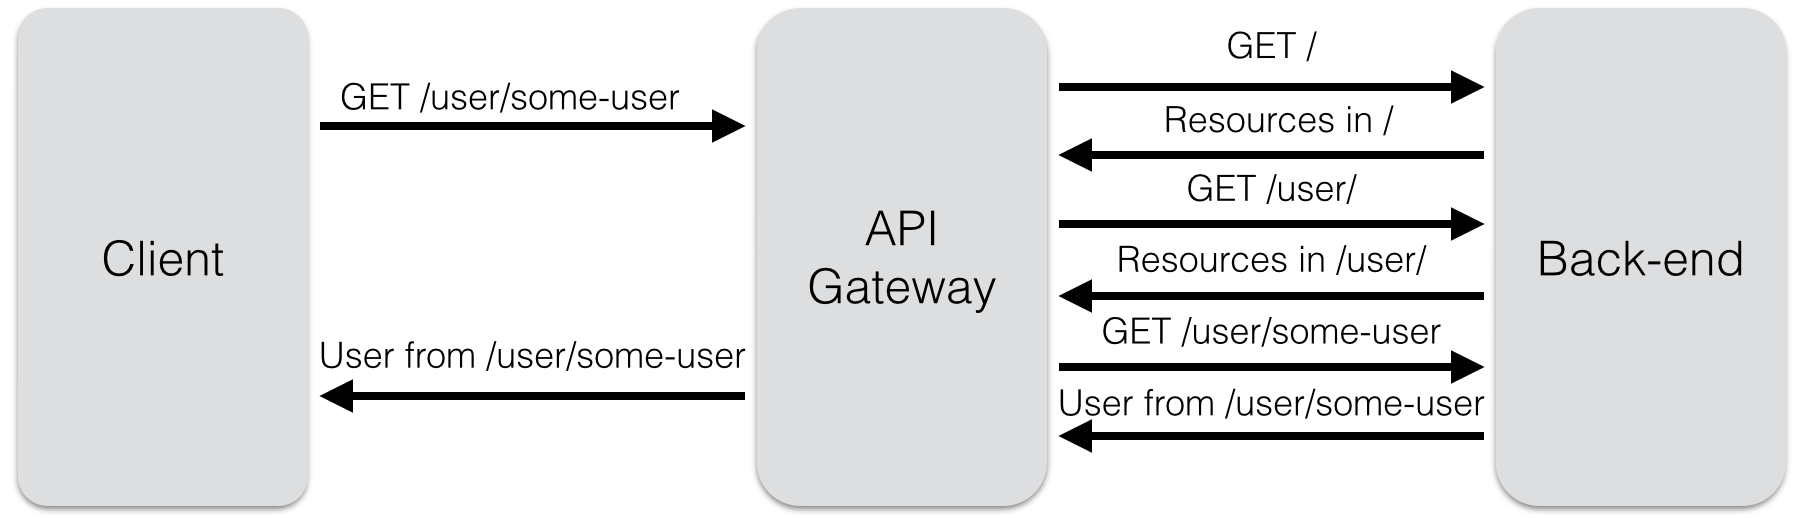
\includegraphics[width=0.9\textwidth]{images/api_gateway_hateoas.png}
    \end{center}
  \caption{Scenario where the API gateway performs the pure REST HATEOAS-communication and at the same time exposes a simple end-point for the client.}
\end{figure}

\section{Compression}
API gateways can be used to compress responses in the cases where no compression is present on the back-end API. This can significantly reduce the amount of traffic the client has to receive which increases the performance - especially on mobile devices. HTTP compression was explored on page \pageref{compression} where it was noted that Gzip has an expected compression level of 60-80\% on text-based files.

\begin{figure}[H]
  \centering
    \begin{center}
      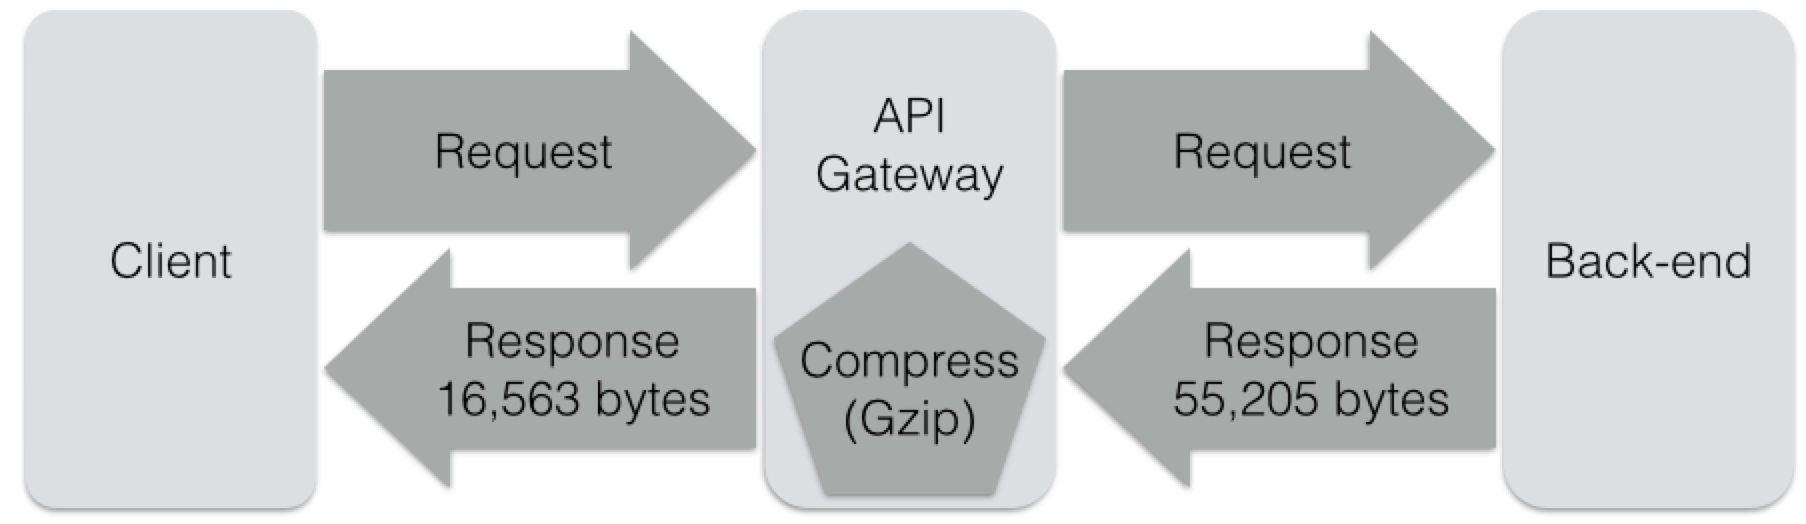
\includegraphics[width=0.9\textwidth]{images/api_gateway_compression.png}
    \end{center}
  \caption{The API gateway compresses the response from the back-end API with Gzip which reduces the response traffic in the client by 70\%. Numbers taken from the example on page \pageref{compression}.}
\end{figure}

\section{Caching}
Responses from frequent API calls can be cached in the API gateway to reduce the load on the back-end system\cite[page 107]{AASG}. The cache can have a specified lifetime or be invalidated based on certain events such as a table update on a database.

\begin{figure}[H]
  \centering
    \begin{center}
      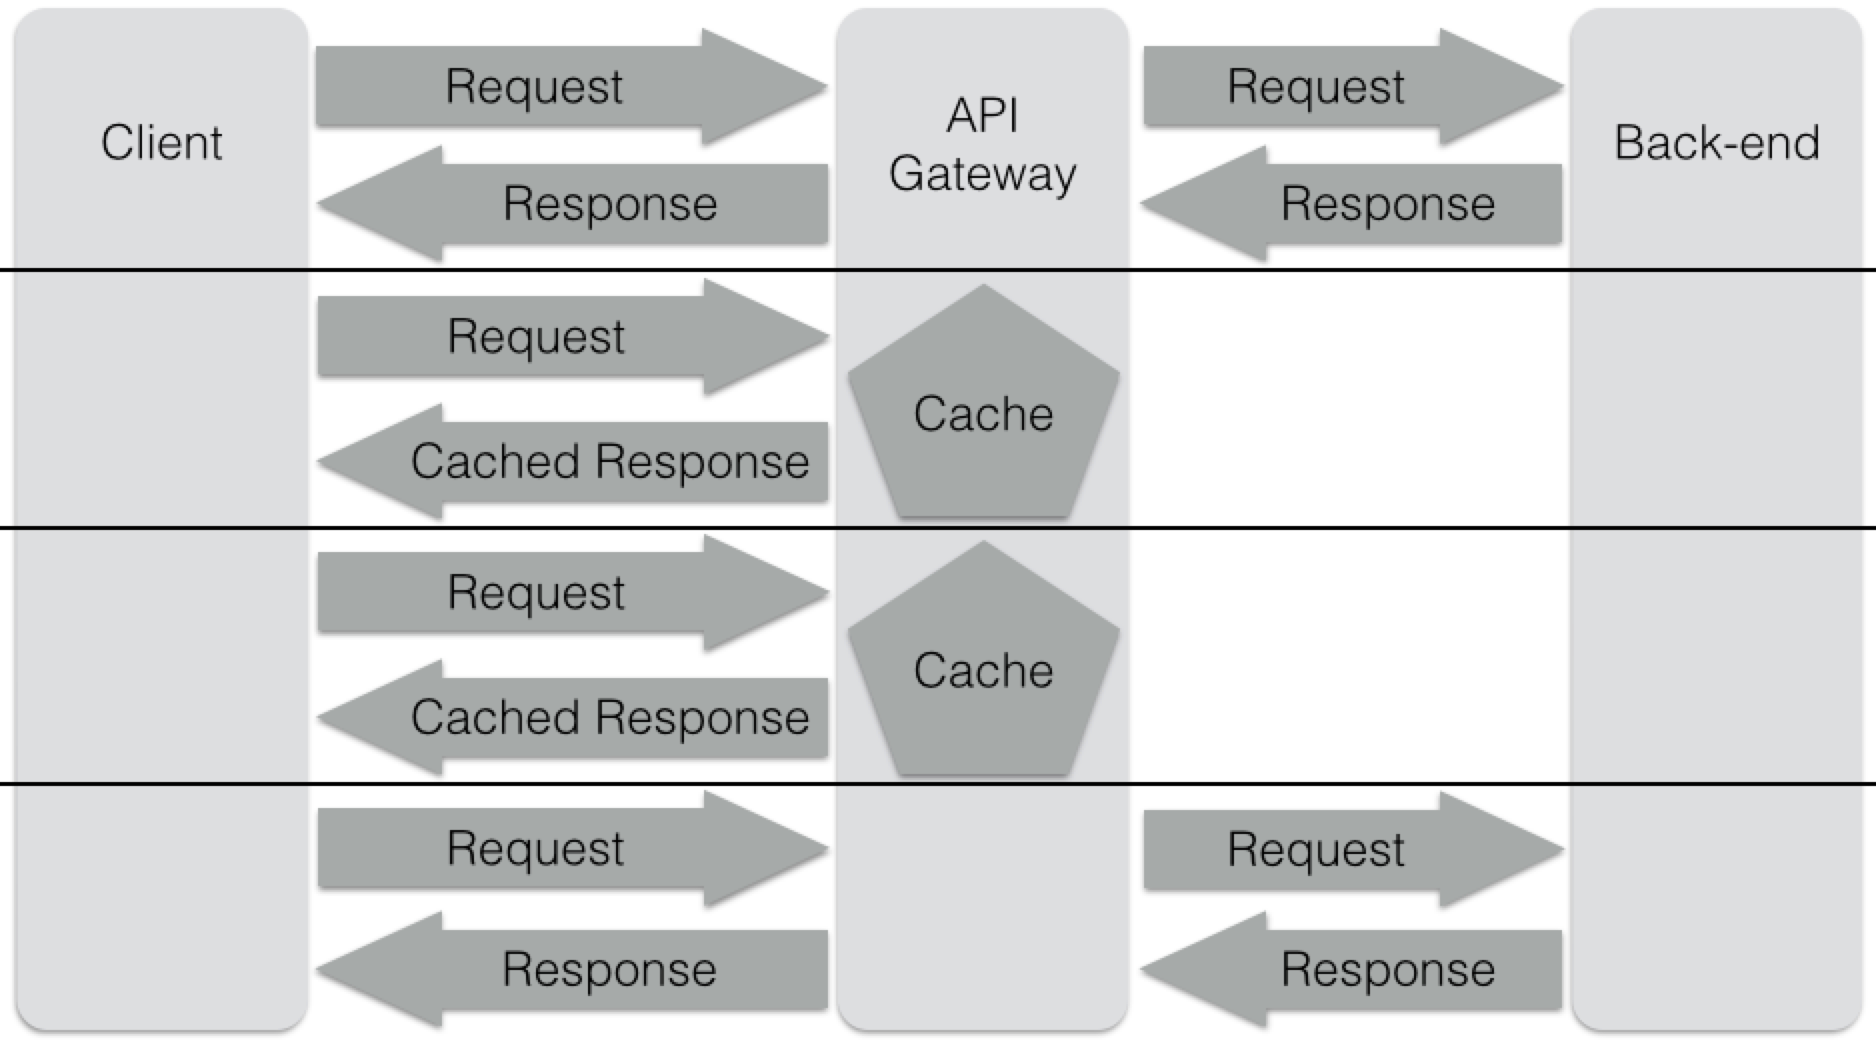
\includegraphics[width=0.9\textwidth]{images/api_gateway_cache.png}
    \end{center}
  \caption{Frequent API calls to the same end-point can be cached to reduce the load on the back-end.}
\end{figure}

\section{Decreasing bandwidth \& cost}
Cloud providers, such as Amazon\cite{cloud_amazon} and Microsoft\cite{cloud_microsoft}, does not charge for bandwidth as long as data is transfered between servers in the same regions. When using an API-gateway in the cloud, bandwidth \& its costs can be reduced by placing the API-gateway in the same cloud region and apply bandwidth saving techniques such as the previously in this chapter mentioned: compression, duplicate \& unnecessary items, pure REST and in some cases even format transformation.

\begin{figure}[H]
  \centering
    \begin{center}
      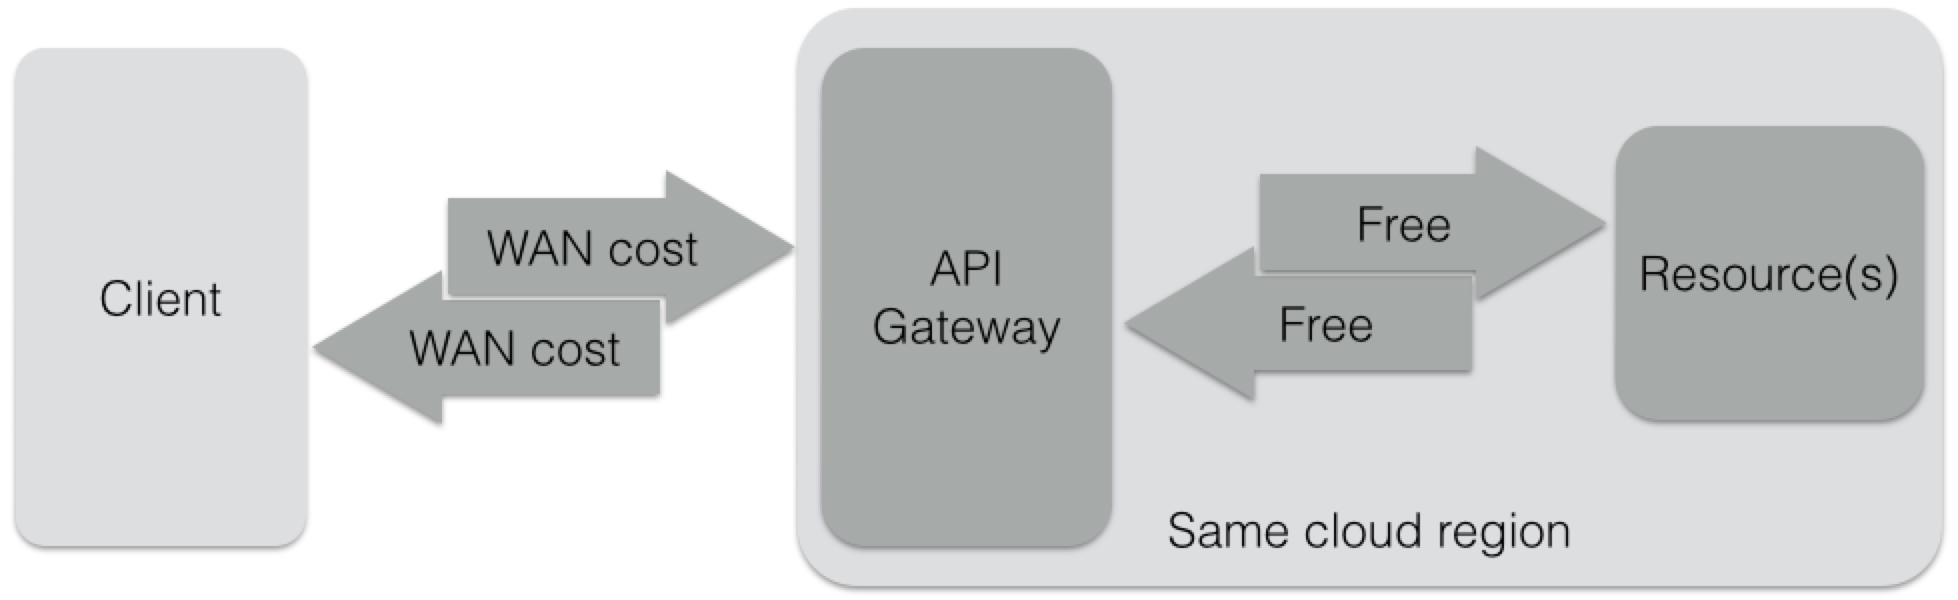
\includegraphics[width=0.9\textwidth]{images/api_gateway_bandwidth.png}
    \end{center}
  \caption{How cloud providers such as Amazon\cite{cloud_amazon} and Microsoft\cite{cloud_microsoft} charges based if the traffic is over WAN or in the same cloud region.}
\end{figure}

\section{Latency}

\section{Authentication}

\section{Support older API versions}

\section{SSL}

\section{Metrics \& analytics}

\chapter{Crocodile Pear - API-gateway prototype}

\section{Language \& Libraries}
\subsection{Elixir}
Elixir is a functional language designed for building scalable and maintainable applications on the Erlang Virtual Machine. The Erlang VM is known for running low-latency, distributed and fault-tolerant systems while also being successfully used in web development\cite{elixir}. Properties all of which are important for a successful API-gateway implementation.

Two other important influences for choosing Elixir in this prototype are the pipe operator and the asynchronicity achieved by utilising Elixir processes.

\subsection{The pipe operator}
One of the integral parts of Elixir is the pipe operator: $|>$. The pipe operator takes the output from the expression left side of the operator and pipes it into the first argument of the right hand side function. People who are accustomed to Unix may see the similarity with the Unix pipe operator: $|$.

As an example, we can take a look at the following hard to read code:

\begin{figure}[H]
  \centering
\begin{lstlisting}[breaklines=true,frame=single]
Enum.sum(Enum.filter(Enum.map(1..100_000, &(&1 * 3)), odd?))
\end{lstlisting}
  \caption{Elixir code written without the pipe operator.}
\end{figure}

The code from the figure above can be rewritten using the pipe operator which results in a more easily read version:

\begin{figure}[H]
  \centering
\begin{lstlisting}[breaklines=true,frame=single]
1..100_000 |> Stream.map(&(&1 * 3)) |> Stream.filter(odd?) |> Enum.sum
\end{lstlisting}
  \caption{The same Elixir code written with the pipe operator.}
\end{figure}

This also makes you read and reason about the code in a better way. Wehn you read it, you might say something like: "First I have the range of numbers, then I map over it, then I filter them, then I sum them".

The pipe operator is also an important part in how Crocodile Pear works, as it pipes requests to a result, potentially through transformations along the way.

\subsection{Elixir processes}
Processes are Elixir's term for using the Actors model for its concurrency model. In Elixir, processes are extremely lightweight (compared to operating system processes) which means that it is not uncommon to have thousands of them running simultaneously. They run concurrently, isolated from each other and can only communicate by message passing\cite{elixir_processes}.

\subsection{Plug}
Plug is a specification for composable modules in between web applications - and works as connection adapters for different web servers in the Erlang VM\cite{plug}. In Crocodile Pear, Plug is utilised for exposing an end-point for the clients and way for them to receive responses over HTTP for their requests.

\subsection{HTTPoison}
Internally, Crocodile Pear uses HTTPoison\cite{httpoison}. It is based on hackney\cite{hackney}, and is used for executing HTTP requests. The HTTPoison library are only strictly used internally and it is abstracted away to ensure that it can be removed or replaced in the future. 

\section{High-level concept}

\subsection{Data}
The data used in Crocodile Pear corresponds to that of an HTTP request. It consists of a numeric HTTP code, such as 200 for OK, headers which is an key-value map and an arbitrary amount of chunks which makes up the actual data payload of the HTTP request/response - in this document called the body (not to be confused with the HTML body-tag).

\subsection{Producer \& Consumer}
The key component in Crocodile Pear's asynchronous behaviour is the relationship between producers and consumers. Both consumers and producers as fully asynchronous Elixir processes which communicate by passing messages. When a consumer is ready to receive data from a producer, it sends a message to the producer with its identity and a status telling the producer that it is ready to receive.

\begin{figure}[H]
  \centering
\begin{lstlisting}[breaklines=true,frame=single]
send(producer, { :ready, self })	
\end{lstlisting}
  \caption{The consumer sends a tuple with status "ready" and the identity of itself, using the function self(), to the producer when it is ready to receive data.}
\end{figure}

The identity of the producer is always known to the consumer via an Elixir PID, process identification, which is passed around in the pipeline (explained below). The producer will only produce a response once and will terminate after a consumer has consumed the response.

\begin{figure}[H]
  \centering
    \begin{center}
      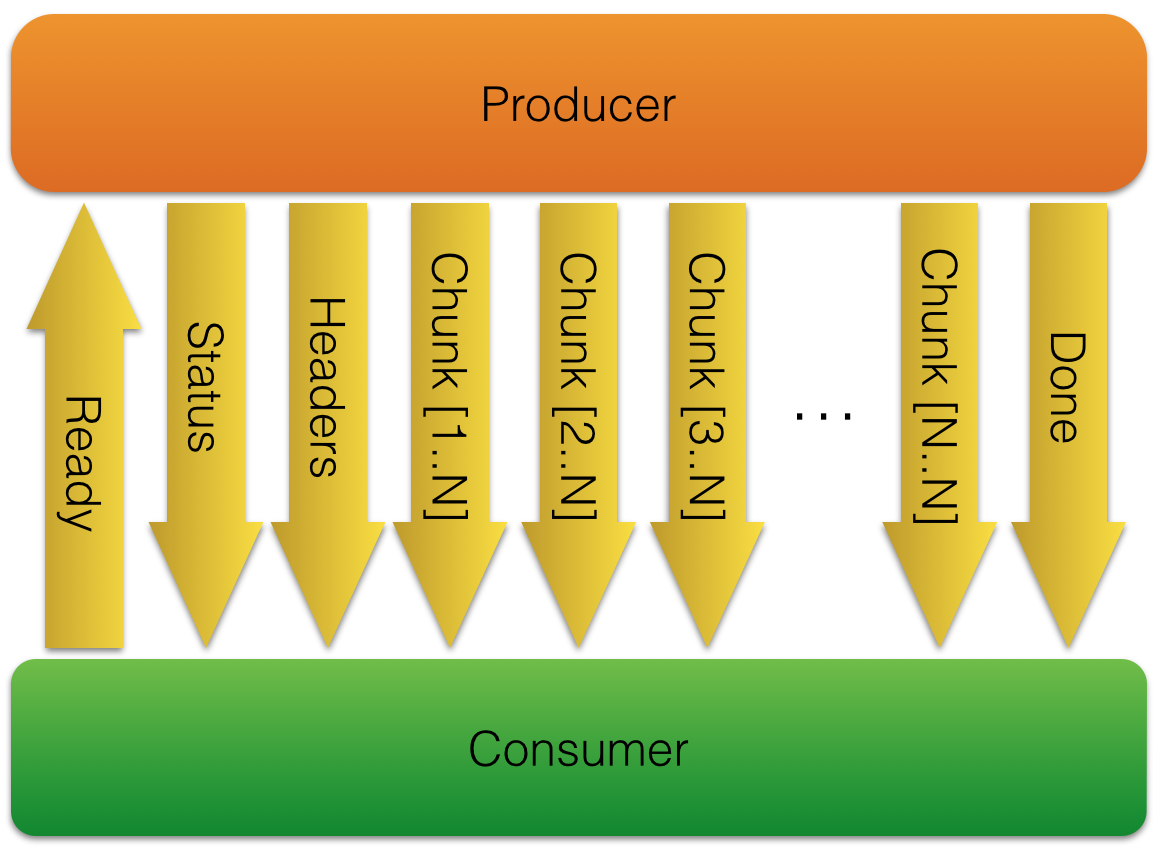
\includegraphics[width=0.9\textwidth]{images/crocpear_producer_consumer.png}
    \end{center}
  \caption{Message passing between a producer and a consumer. Time goes from left to right.}
\end{figure}

After the producer has been notified that a consumer is ready to consume its data, it must first respond with the status and the headers. After that, the chunks must be sent in order. Finally, a done message is sent indicating that the producer will terminate and all chunks have been sent.

\section{Pipeline}
The pipeline is what ties all parts in Crocodile Pear together. The pipeline follows a simple rule: every intermediate function should take a list of producer PIDs as its first argument and return a new list of producer PIDs.

The two exceptions are the two functions $request$ and $response$ which is the beginning and the end of a pipeline.

\subsection{Request}
The $request$ function in Crocodile Pear takes one URI, or a list of URIs, and will always return a list of producer PIDs. Each producer will produce the result of an HTTP request to the specified URI.

\subsection{Response}
The $response$ function takes a list of producers and turns this in to an HTTP response by utilising the provided $conn$ in $Plug$. If more than one producer is passed to the $response$ function, the first responding producer will be consumed first which means that the response order is not deterministic. However, the first responding producer will be consumed until fully completed before any other producer is consumed which guarantees that the chunks will not be mixed together.

As soon as a chunk from a producer has been consumed by the response function, it will respond to the client with the consumed chunked via a chunked HTTP response.

\subsection{Transformers}
Transformers is a concept used in Crocodile Pear to manipulate the data when it flows between one, or several, request(s) and a response,

A transformer function takes a lambda function as its parameter. This lambda function pattern matches on the three types of messages: the status, the header-map and the combined chunks, the actual payload denoted body, and applies a function on these parts to manipulate them in some way.

\begin{figure}[H]
  \centering
\begin{lstlisting}[breaklines=true,frame=single]
blanker = fn(response) ->
  case response do
    {:status, _status}  -> 404
    {:headers, _headers} -> %{}
    {:body, _body} -> ""
  end
end
\end{lstlisting}
  \caption{The function blanker is a simple lambda function which can be used in a transformer. It sets the status to 404 and removes all headers and the payload by simply ignoring the received values and providing empty ones instead. The actual data in status, headers and body are discarded by using an underscore at the start of the variables in the pattern matching.}
\end{figure}

\subsection{Timers}
Crocodile Pear include timers which can be placed anywhere in the pipeline to benchmark the time it takes to reach the different stages. They can be used anonymously or with labels attached to them and will output data to the default logger.

However, because of the asynchronous nature of Crocodile Pear, the logged time is when a function has been executed - not when the returned producers has finished executing.

\begin{figure}[H]
  \centering
\begin{lstlisting}[breaklines=true,frame=single]
12:12:28.719 [info]  {1424, 171548, 716696} (Got URL)
12:12:28.724 [info]  {1424, 171548, 721651} (Executed request)
12:12:29.753 [info]  {1424, 171549, 753316} (Collected response)
12:12:29.753 [info]  {1424, 171549, 753396} (Got body)
12:12:29.763 [info]  {1424, 171549, 763664} (Decoded JSON)
12:12:29.763 [info]  {1424, 171549, 763702} (Extracted data)
12:12:29.764 [info]  {1424, 171549, 763987} (Mapped image url)
12:12:29.764 [info]  {1424, 171549, 764107} (Executed request)
12:12:29.765 [info]  {1424, 171549, 765113} (Added transform function)
12:12:30.700 [info]  {1424, 171550, 700280} (Responded to query)
\end{lstlisting}
  \caption{The output from the logger. From left to right: time when message is logged, log level, Erlang timestamp \{MegaSecs, Secs, Microsecs\}, optional message.}
\end{figure}

Bättre asynkron mätning kanske kommer fixas?!

\subsection{Concatenate JSON}
The function $concatenate\_json$ takes a list of producers, consumes them and returns a new producer. The new producers chunks will be the responses from the previous consumers, concatenated to a JSON list. Each chunk sent by the new producer will be one item from the JSON list, along with some JSON syntactical data.

Each item in the list will be a JSON-object containing the three keys: status, headers and body (payload). Optionally, if a "true" value is passed in to the function, each item in the list will be only the "body" (payload) with the headers and status omitted.


\begin{figure}[H]
  \centering
    \begin{center}
      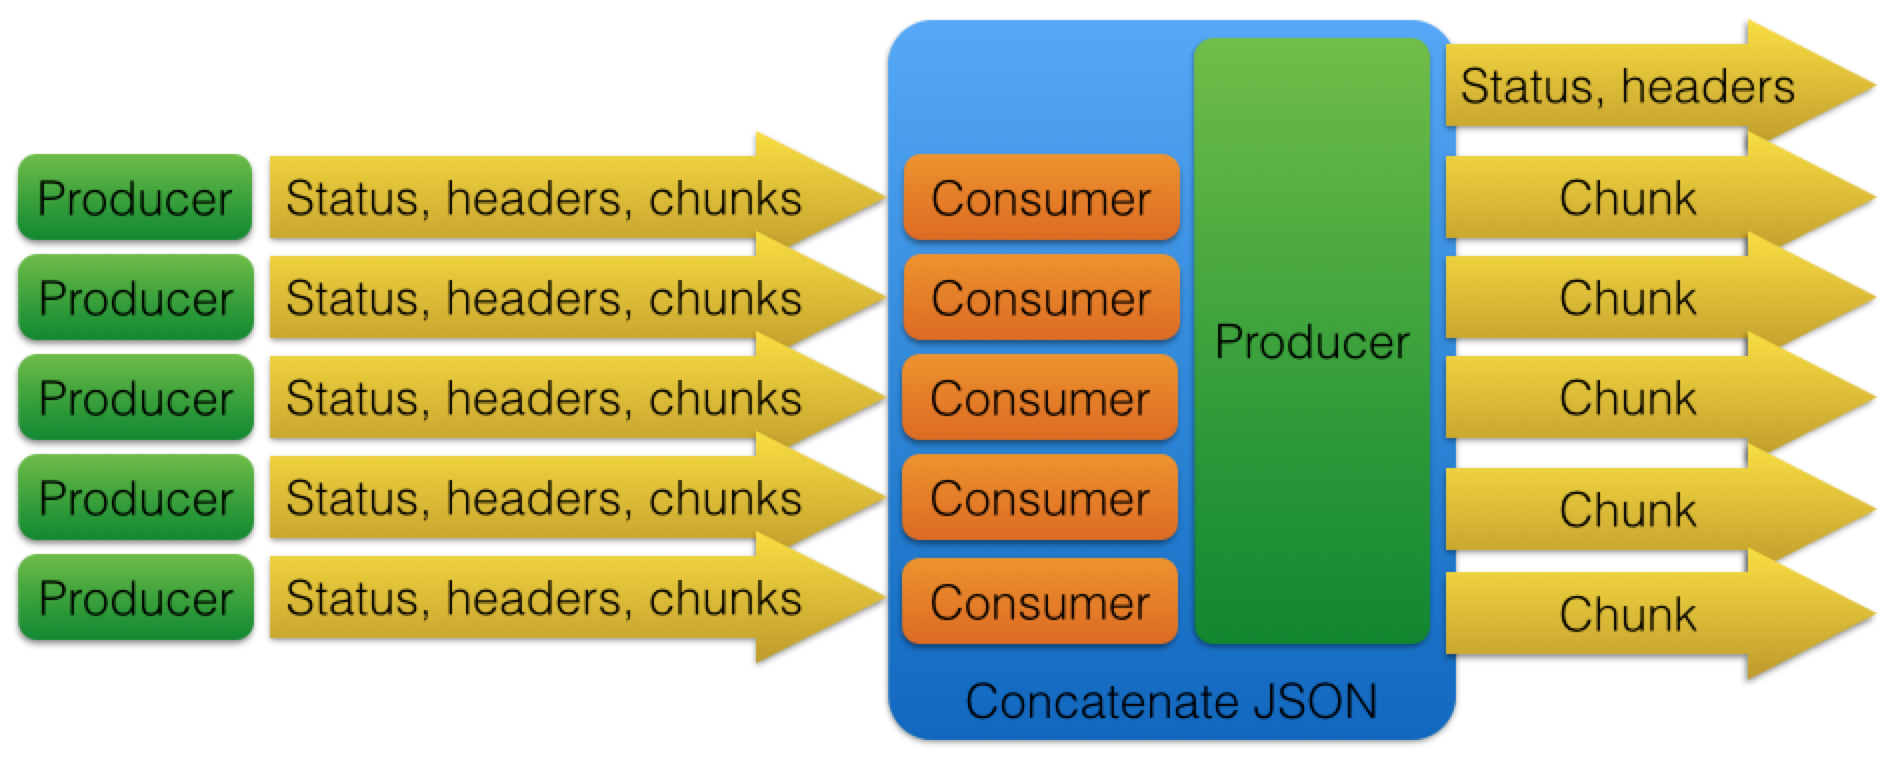
\includegraphics[width=0.9\textwidth]{images/crocpear_concatenate_json.png}
    \end{center}
  \caption{Concatenate JSON creates one consumer for each producer. As soon as one consumer has consumed an entire response, the new producer will send that as a chunk in JSON format.}
\end{figure}

Even though $concatenate\_json$ takes an arbitrary number of producer PIDs as its argument, it will itself only return one new producer as its result is one JSON list object.


\section{Examples}
\subsection{Request proxying}
A simple proxy is a good introductionary example which demonstrates how the request / response pipeline can be used. In this example, we extract an URI from the query string in the connection and pipe it to the $request$ function which in turn is piped into the $response$ function.

\begin{figure}[H]
  \centering
\begin{lstlisting}[breaklines=true,frame=single]
conn.query_string
|> request
|> response(conn)
\end{lstlisting}
  \caption{A simple proxy.}
\end{figure}

In a similar fashion, we could take an arbitrary number of requests and proxy them into one result. Here we take several URIs from the query string, separated by the character "|" and pipe them in to the $request$ and $response$ as before. By using Elixirs String.split, a list of strings is created which is passed into the $request$ function.

\begin{figure}[H]
  \centering
\begin{lstlisting}[breaklines=true,frame=single]
String.split(conn.query_string, "|")
|> request
|> response(conn)
\end{lstlisting}
  \caption{A simple proxy for an arbitrary number of URIs.}
\end{figure}

This will execute all requests concurrently and start responding, in indeterministic order, based on which of the requests is responding first.

\subsection{Concatenate responses to JSON}
The concatenate\_json function can be used to concatenate several requests into a JSON list object. It will also set the "Content-Type" header to the appropriate "application/json".

\begin{figure}[H]
  \centering
\begin{lstlisting}[breaklines=true,frame=single]
String.split(conn.query_string, "|")
|> request
|> concatenate_json
|> response(conn)
\end{lstlisting}
  \caption{Demonstration of the concatenate\_json function.}
\end{figure}

The response will be one JSON list containing response's status, headers and payload as JSON objects.

\subsection{Transformers}
In this more complex example, we will use all previously explained techniques along with a transformer to create a more powerful end-point. We will go over the code in the following figure line by line.

\begin{figure}[H]
  \centering
\begin{lstlisting}[breaklines=true,frame=single]
uris =
  String.split(conn.query_string, "|")
  |> Enum.map(&("http://api.openweathermap.org/data/2.5/weather?q=#{&1}"))

temperature_extractor = fn(item) ->
  case item do
    { :body, body } ->
      response_body = Poison.decode!(body)

      Map.put(%{}, response_body["name"], response_body["main"]["temp"])
      |> Poison.encode!

    { _other, other } -> other
  end
end

uris
|> request
|> transform(temperature_extractor)
|> concatenate_json(true)
|> response(conn)
\end{lstlisting}
  \caption{A complex example with a transformer.}
\end{figure}

On line 1 - 3, we intercept cities and country codes, such as "Lund,SE|Copenhagen,DK", from the query string sent through the connection and then split them in to a list using the separating character: $|$. This list is then mapped over which will create appropriate URIs for the underlying API which we will use in this example.

On line 5 - 15, we create a new transformer lambda function. When we receive the actual payload data, the body, we will decode it from JSON format to native Elixir data types using the third-party library Poison\cite{poison}. We will transform the responses and create a new JSON object by extracting the name and temperature as a new key-value pair and encode it using Poison again - all other payload data is discarded. The other data, status and headers, will be left intact by defining that "other" returns itself, "other".

On line 17 - 21, we tie everything together using the pipeline. We take the URIs, pipe them into a request, pipe the request in to a transformer with our new function, pipe that in to the concatenate\_json function and pipe that to the response.

In this example, we have used response concatenation, discarding of duplicate and unnecessary data, and provided a simple way for clients to request temperature data from multiple cities in one requests with a tailor made response.

\subsection{Timers}
Timers can be used anywhere in the pipeline to output timed logger information.

\begin{figure}[H]
  \centering
\begin{lstlisting}[breaklines=true,frame=single]
uris
|> timer("got URIs")
|> request
|> timer("created requests")
|> transform(temperature_extractor)
|> timer("added transformer")
|> concatenate_json(true)
|> timer("concatenated to JSON")
|> response(conn)
|> timer("started responding")
\end{lstlisting}
  \caption{Using timers in the pipeline.}
\end{figure}

The logger would then give the following output:

\begin{figure}[H]
  \centering
\begin{lstlisting}[breaklines=true,frame=single]
13:46:53.625 [info]  {1424, 177213, 625128} (got URIs)
13:46:53.625 [info]  {1424, 177213, 625228} (created requests)
13:46:53.625 [info]  {1424, 177213, 625576} (added transformer)
13:46:53.626 [info]  {1424, 177213, 625658} (concatenated to JSON)
13:46:53.735 [info]  {1424, 177213, 735330} (started responding)
\end{lstlisting}
  \caption{How the timer would log during the pipeline.}
\end{figure}

\cleardoublepage
\phantomsection
\addcontentsline{toc}{chapter}{Bibliography}
\bibliographystyle{plain}
\bibliography{anton_msc}

%\makebibliography{anton_msc}

\end{document}